\documentclass[platex,dvipdfmx,a4paper,twocolumn,base=8.5pt,jbase=8.5pt,ja=standard]{jsarticle}

\usepackage[top=30truemm,bottom=25truemm,left=20truemm,right=20truemm]{geometry}
\usepackage[dvipdfmx]{graphicx,color}
\usepackage{cite}
\usepackage{array}
\usepackage{float}
\usepackage{subcaption}
\usepackage{amsmath}
\usepackage{ipsj}


% 画像ファイルのパスを設定(srcディレクトリ基準とoutディレクトリ基準の両方を追加)
\graphicspath{{../src/pictures/}{pictures/}}

\pagestyle{empty}
\setlength{\columnsep}{7mm}

%\setlength{\textfloatsep}{6pt plus 2pt minus 2pt}
%\setlength{\intextsep}{6pt plus 2pt minus 2pt}
%\setlength{\abovecaptionskip}{2pt}
%\setlength{\belowcaptionskip}{2pt}
%\setlength\textfloatsep{15pt}


\usepackage{indentfirst}  % プリアンブルに追加

% セクション周りの余白設定
\makeatletter
% \section の前後の余白
% セクション後の段落もインデントする
\@afterindenttrue

\makeatother


\titlespacing{\subsection}
{0pt}% left
{6pt}% before-sep
{1.2pt}% after-sep
\setlength\textfloatsep{15pt}
\title{VR酔い低減を目的とした三感覚系のマルチモーダル刺激システム}{A Multimodal Stimulation System Targeting Three Sensory Systems for VR Motion Sickness Reduction}

\author{横浜国立大学}{高須賀 颯太}{Sota Takasuga, Yokohama National University}
\author{横浜国立大学}{竹中 健祐}{Kensuke Takenaka, Yokohama National University}
\author{横浜国立大学}{島 圭介}{Keisuke Shima, Yokohama National University}
\author{広島県立大学}{島谷 康司}{Koji Shimatani, Prefectural University of Hiroshima}


\date{}

\begin{document}
    \pagestyle{empty}  % ページ番号を消す
    \setlength{\abovedisplayskip}{-3pt} % 上部のマージン
    \maketitle
    \thispagestyle{empty}  % 最初のページのページ番号も消す(maketitleの後に配置が重要)


    \section{はじめに}
    頭部装着型ディスプレイ (HMD) を用いた仮想現実(VR)は訓練・設計支援・教育など多様な領域へ普及しているものの,利用継続を妨げる要因としてVR酔いが知られている\cite{Saredakis2020Factors}.VR酔いは視覚運動により生じた自己運動知覚に対し,前庭・体性感覚が不整合である場合に生じやすく,吐き気やめまい等のを引き起こす.
    これに対し,前庭感覚または体性感覚に刺激を与えることでVR酔いの低減や没入感向上を図る手法が提案されている\cite{Sra2019ProprioGVS,Peng2020WalkingVibe}.一方で,単一の感覚刺激のみでは視覚運動との整合が不十分となる可能性がある.そのため前庭電気刺激 (Garvanic Vestibular Stimulation : GVS) と振動刺激の重畳提示が有望と考えられるが,その効果は十分に検証されていない.


    そこで本稿では,視覚運動に同期したGVSと頬・首への振動刺激を組み合わせて提示することで,加速度感覚の補完と感覚間整合の向上を狙う.提案システムではVR上の速度・加速度に基づきマルチモーダル刺激を同期制御するシステムを構築し,VR酔いの低減と没入感の向上効果を評価する.


    \section{提案システム}
    図\ref{fig:system_photo}に提案法の概要を示す.提案システムでは,VRシミュレーション上で生じる速度$v$,加速度$a$から,それぞれの感覚刺激量を算出し,開発した刺激デバイスを用いて感覚を提示する.



    \subsection{ハードウェア}
    刺激デバイスは大きく分けてGVS用電流出力部,振動用駆動部から構成される.PCから送信される右振動・左振動・GVSの3つの刺激量を受信し,視覚運動に同期したマルチモーダル刺激を実現する.

    振動刺激部には振動子 (フォスター電機社製) を用い,左右の頬および首周辺に配置し,それぞれ独立に駆動する.GVSはオペアンプを用いた定電流回路を用い、乳突部に貼付した電極を介して提示する.出力できる最大電流は3.3 mAである.以上により,本デバイスは前庭電気刺激(電流)と体性感覚刺激(左右振動振幅)を同時に提示可能である.

    また,ユーザが不快に感じない最大刺激量として,GVSの最大電流$I_{\rm max}$と振動の最大振幅$U_{\rm max}$を予め設定し,ソフトウェア上で算出される無次元の指令値(GVS:$i(t)$,振動:$u_{\rm R}(t),u_{\rm L}(t)$)を乗算した刺激量を与えることで,被験者ごとに最適化した感覚刺激を提示する.
    \begin{figure}[t]
        \centering
        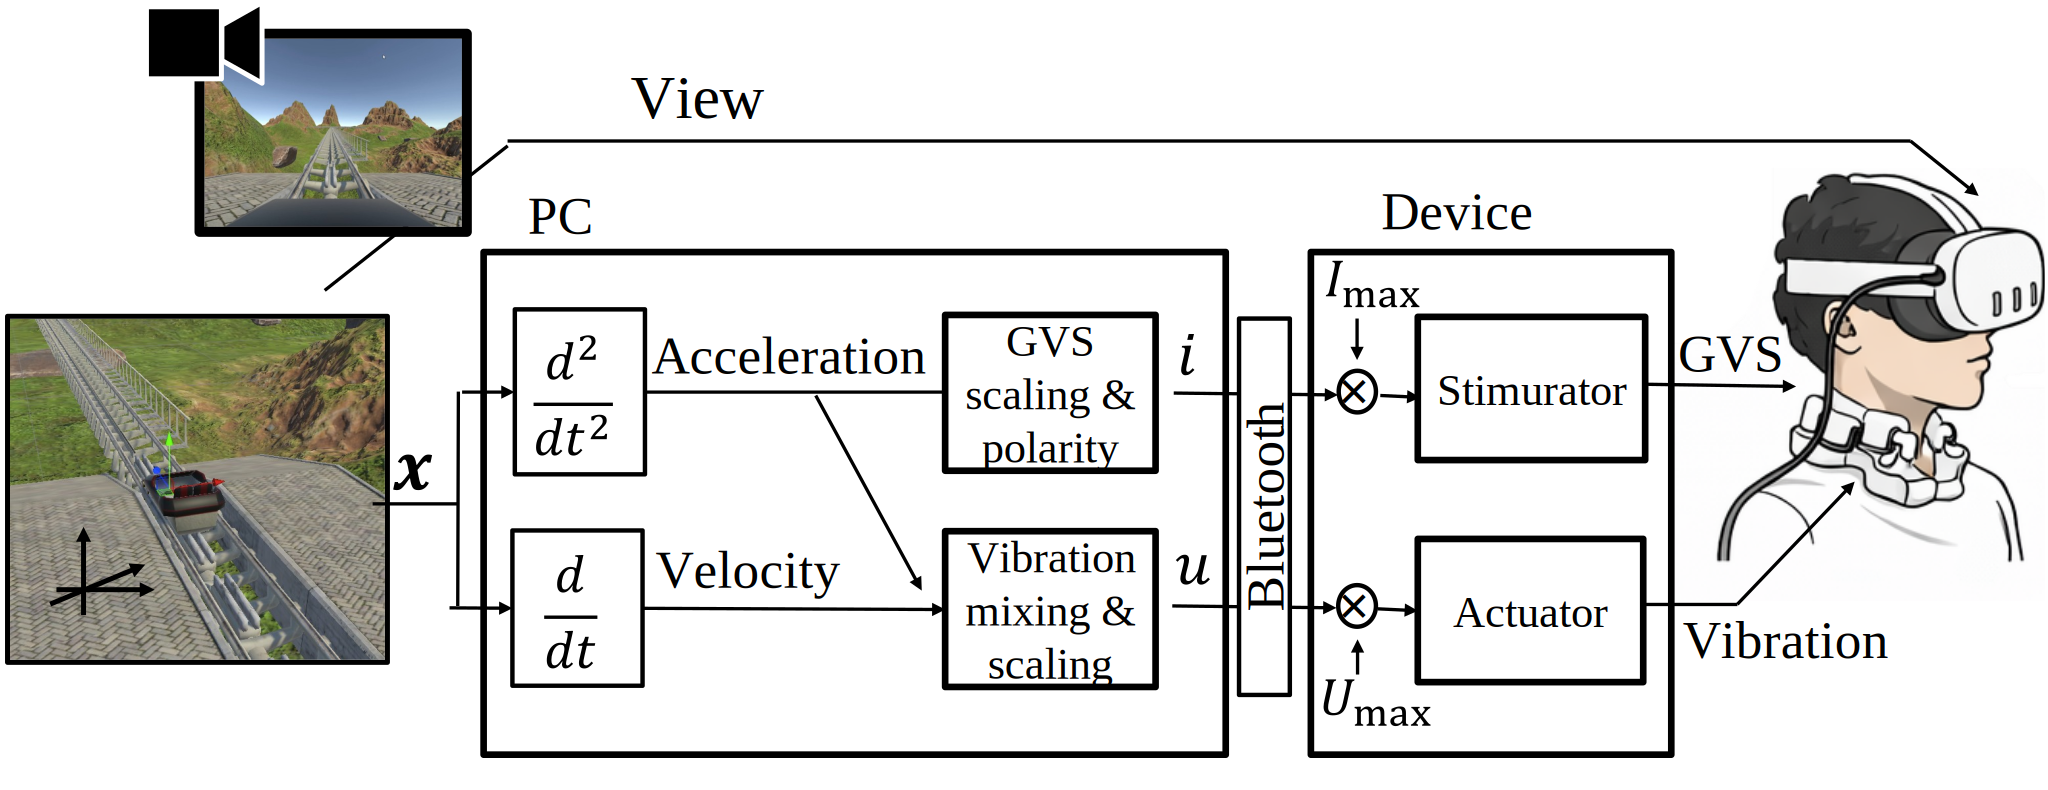
\includegraphics[width=0.95\columnwidth]{image.svg}
        \caption{提案システム}
        \label{fig:system_photo}
    \end{figure}

    \subsection{ソフトウェア}
    提案法では,仮想空間上の視点位置$\boldsymbol{x}(t)$から,その時間微分により速度,二階微分により加速度を算出する.
    \begin{equation}
        \boldsymbol{v}(t)=\frac{d \boldsymbol{x}(t)}{dt},\qquad
        \boldsymbol{a}(t)=\frac{d^2 \boldsymbol{x}(t)}{dt^2}
    \end{equation}


    GVSでは,加速度に比例してGVS指令値を生成する.スケーリング係数$k_{\rm a}$を用いて
    \begin{equation}
        i(t)=k_{\rm a}\,a(t)
    \end{equation}
    とし,最終的な電流は次式で与える.
    \begin{equation}
        I(t)=I_{\rm max}\,i(t)
    \end{equation}

    振動刺激は左右のアクチュエータを独立に駆動する.速度の大きさ$|v_{\rm fwd}(t)|$と加速度$a(t)$を混合して振幅指令値を生成する.混合比$r$(速度側の重み)およびスケーリング係数$k_{\rm v}$を用いて
    \begin{align}
        u_{\rm R}(t) &= (1-r)\,i(t) + r\,k_{\rm v}\,|v_{\rm fwd}(t)|, \\
        u_{\rm L}(t) &= -(1-r)\,i(t) + r\,k_{\rm v}\,|v_{\rm fwd}(t)|
    \end{align}
    とする.最終的な振動刺激量は
    \begin{equation}
        U_{\rm R}(t)=U_{\rm max}\,u_{\rm R}(t),\qquad
        U_{\rm L}(t)=U_{\rm max}\,u_{\rm L}(t)
    \end{equation}
    とし,右・左の振動アクチュエータを駆動する.



    \section{実験}
    前庭・体性感覚の重畳刺激によるVR酔いの低減と没入感の向上の検証のため,健常若年者8名 (平均22.5歳$\pm 1.5$歳) に対して実験を行った。

    被験者はHMDを装着し,Unity上で提示されるコースター体験タスクを実施した.タスク時間は1分とし,簡易化のため視点運動は左右方向の運動成分のみを持つように設計した.図\ref{fig:exp_task}に被験者装着の様子とタスク画面を示す.また,$I_{\rm{max}} = 2 \; \rm{mA}, U_{\rm{max}} = 10 \; \rm{mm},  k_{\rm a} = 1,  k_{\rm v} = 1,  r = 0.7$とした.

    \begin{figure}[tbp]
        \centering
        \begin{subfigure}[b]{0.48\columnwidth}
            \centering
            \includegraphics[width=\linewidth]{exp_subject.png}
            \caption{被験者装着の様子}
            \label{fig:exp_subject}
        \end{subfigure}
        \hfill
        \begin{subfigure}[b]{0.48\columnwidth}
            \centering
            \includegraphics[width=\linewidth]{exp_scene.png}
            \caption{Unity上のタスク画面}
            \label{fig:exp_scene}
        \end{subfigure}
        \caption{実験環境とタスク}
        \label{fig:exp_task}
    \end{figure}

    実験では前庭電気刺激について無・弱(感覚閾値未満)・強(約$2\;\mathrm{mA}$)の3水準,振動刺激について無・有の2水準とし,$3\times2$の計6条件を設定した.表\ref{tab:conditions}に刺激条件の対応を示す.感覚閾値は被験者ごとに同定し,弱条件は主観的に知覚されない範囲で設定した.強条件は約$2\;\mathrm{mA}$を目安に設定した.各条件は3試行とし,条件順は被験者ごとにランダムに決定した.

    \begin{table}[tbp]
        \centering
        \footnotesize
        \caption{実験条件(刺激条件の対応)}
        \label{tab:conditions}
        \begin{tabular}{c>{\centering\arraybackslash}m{0.42\columnwidth}>{\centering\arraybackslash}m{0.20\columnwidth}}
            \hline
            条件 & 前庭電気刺激(GVS)          & 振動刺激 \\
            \hline
            a  & 無                    & 無    \\
            b  & 弱(感覚閾値未満)            & 無    \\
            c  & 強(約$2\;\mathrm{mA}$) & 無    \\
            d  & 無                    & 有    \\
            e  & 弱(感覚閾値未満)            & 有    \\
            f  & 強(約$2\;\mathrm{mA}$) & 有    \\
            \hline
        \end{tabular}
    \end{table}

    評価指標としてVR酔いの程度をVirtual Reality Sickness Questionnaire(VRSQ)\cite{Kim2018VRSQ}で評価し,没入感をVisual Analog Scale(VAS)で取得した.個人差を抑えるため,各条件のスコアから条件a(刺激なし)を基準とした差分を算出し,各条件間でボンフェローニ補正を適用した多重比較検定を行った.

    図\ref{fig:vrsq}にVR酔い変化を示す.無刺激(条件a)と比較してGVS弱または振動刺激を付与した条件において有意差が確認された.さらに,片方のみを付与した条件と比較して,両方を併用した条件で有意差が確認され,マルチモーダル刺激による重畳効果が示唆された.

    図\ref{fig:imm}に没入感変化を示す.没入感は刺激条件によって変化し,特に振動刺激を含む条件で向上傾向が見られる.しかしながら個人差や分散が大きくなりやすく,刺激タイミングや強度変調が視覚運動と不整合になる場合には効果が一様にならない可能性がある.したがって,今後は閾値同定や強度スケーリングなどの個人適応を導入し,VR酔い低減と没入感向上の両立を図る必要がある.

    \begin{figure}[tbp]
        \centering
        \begin{subfigure}[b]{0.48\columnwidth}
            \centering
            \includegraphics[width=\linewidth]{VRSQ_diff.png}
            \caption{VR酔い変化}
            \label{fig:vrsq}
        \end{subfigure}
        \hfill
        \begin{subfigure}[b]{0.48\columnwidth}
            \centering
            \includegraphics[width=\linewidth]{immersive_diff.png}
            \caption{没入感変化}
            \label{fig:imm}
        \end{subfigure}
        \caption{VR酔いと没入感の条件別比較}
        \label{fig:results}
    \end{figure}


    \section{おわりに}
    本稿では,視覚運動に同期して前庭電気刺激と頬・首振動を同時制御する加速度感覚誘発システムを提案し,6条件の被験者内比較によりVRSQとVASを用いて評価した.その結果,無刺激条件に対してGVS弱または振動刺激の付与でVR酔い改善に有意差が見られ,さらに単独提示条件に対して併用条件で有意に改善することが確認された.今後は,個人適応を導入し,刺激設計の最適化を進め,幅広いコンテンツや運動条件においても安定して効果を発揮する汎用的な感覚提示手法の確立を目指す.


    % 参考文献の見出しを調整
    \makeatletter
    \renewcommand{\refname}{\normalsize 参考文献}
    \makeatother

    \footnotesize
    \bibliographystyle{junsrt}
    \bibliography{references}
\end{document}
